\documentclass{article}

\usepackage{graphicx}
\usepackage{tikz}
\usepackage{tikzsymbols}
\usetikzlibrary{calc,patterns,shapes.geometric}
\pagestyle{empty}
\usepackage[margin=0pt]{geometry}
\geometry{papersize={14in,12in}}

\def\centerarc[#1](#2)(#3:#4:#5){\draw[#1] ($(#2)+({#5*cos(#3)},{#5*sin(#3)})$) arc (#3:#4:#5);}

\begin{document}
	\begin{figure}
		\centering
		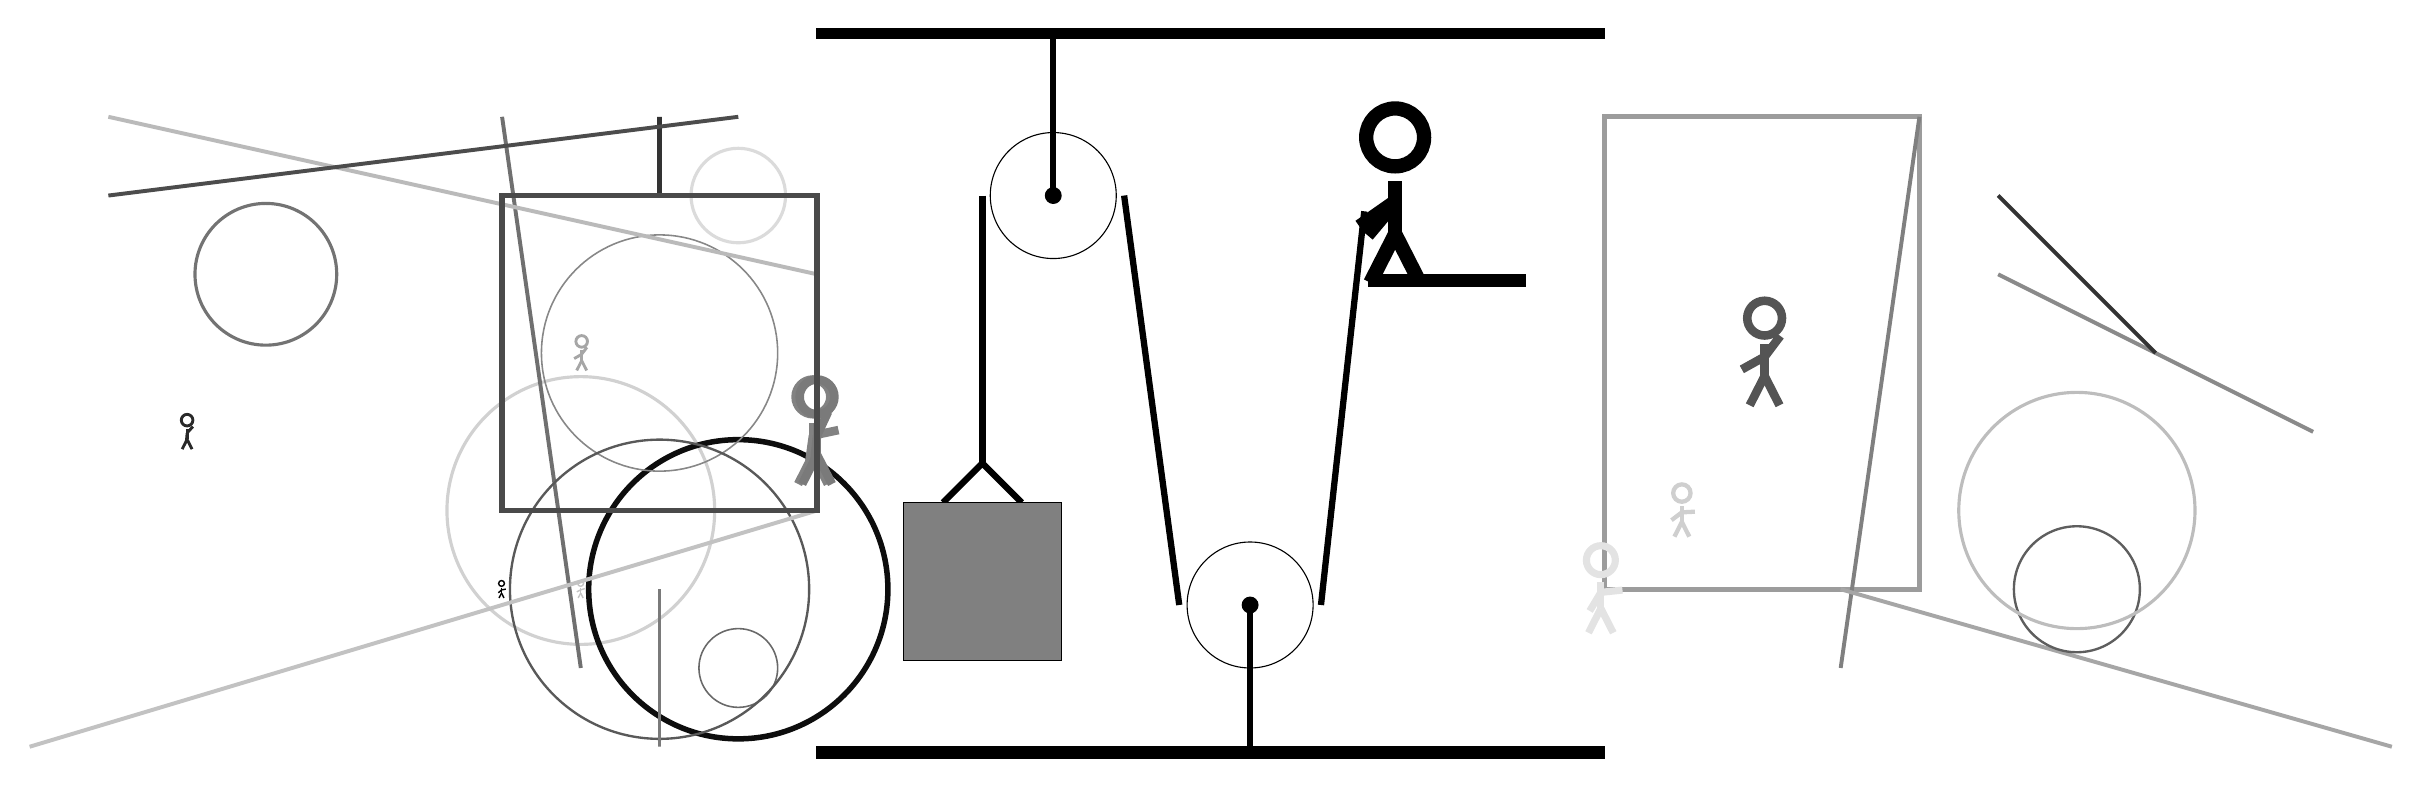
\begin{tikzpicture}
			%%%%% START %%%%%
			
			\draw[fill=black] (-2, 9) rectangle (8, 9.125);
			
			\draw (3.5, 1.8) circle (0.8);
			\draw[fill=black] (3.5, 1.8) circle (0.1);
			\draw[line width=0.8mm] (3.5, 1.8) -- (3.5, 0);
			
			\draw (1, 7) circle (0.8);
			\draw[fill=black] (1, 7) circle (0.1);
			\draw[line width=0.8mm] (1, 9) -- (1, 7);
			
			\draw[line width=0.8mm](-0.4, 3.1) --  (0.1, 3.6) -- (0.6, 3.1);
			\draw[fill=black!50] (-0.9, 3.1) rectangle (1.1, 1.1);
			
			\draw[line width=0.8mm](0.1, 7) -- (0.1, 3.6);
			\centerarc[line width=0.8mm](1, 7)(180:0:0.9)
			\draw[line width=0.8mm](1.9, 7) -- (2.6, 1.8);
			\centerarc[line width=0.8mm](3.5, 1.8)(180:360:0.9)
			\draw[line width=0.8mm](4.4, 1.8) -- (4.95, 6.8);
			
			\node[line width=0.3mm, color=black!100] at (-6, 2) {\Strichmaxerl[1][43][10]};
			
			\node[line width=0.4mm, color=black!19] at (9, 3) {\Strichmaxerl[3][37][3]};
			\draw [line width=0.4mm, color=black!18](-5, 3) circle (1.7);
			\draw [line width=0.2mm, color=black!59](-3, 1) circle (0.5);
			
			\draw [line width=0.7mm, color=black!95](-3, 2) circle (1.9);
			
			\draw[line width=0.6mm, color=black!39] (8, 8) rectangle (12, 2);
			\draw [line width=0.2mm, color=black!47](-4, 5) circle (1.5);
			
			\draw[line width=0.5mm, color=black!56](-6, 8) -- (-5, 1);
			\node[line width=0.5mm, color=black!49] at (-2, 4) {\Strichmaxerl[6][82][12]};
			\draw[line width=0.7mm, color=black!80] (-4, 8) rectangle (-4, 7);
			\node[line width=0.6mm, color=black!23] at (-5, 2) {\Strichmaxerl[1][28][17]};
			
			\draw[line width=0.5mm, color=black!50](12, 8) -- (11, 1);
			\draw [line width=0.3mm, color=black!65](-4, 2) circle (1.9);
			
			\draw[line width=0.5mm, color=black!46](13, 6) -- (17, 4);
			\draw[line width=0.5mm, color=black!24](-2, 3) -- (-12, 0);
			\draw[line width=0.5mm, color=black!35](11, 2) -- (18, 0);
			
			\draw[line width=0.5mm, color=black!80](13, 7) -- (15, 5);
			
			\draw [line width=0.4mm, color=black!14](-3, 7) circle (0.6);
			\draw[line width=0.3mm, color=black!52] (-4, 2) rectangle (-4, 0);
			\node[line width=0.2mm, color=black!11] at (8, 2) {\Strichmaxerl[5][59][6]};
			\draw [line width=0.4mm, color=black!55](-9, 6) circle (0.9);
			
			\node[line width=0.6mm, color=black!52] at (-2, 4) {\Strichmaxerl[6][84][65]};
			
			\draw [line width=0.3mm, color=black!63](14, 2) circle (0.8);
			\node[line width=0.4mm, color=black!67] at (10, 5) {\Strichmaxerl[6][29][53]};
			\draw [line width=0.4mm, color=black!26](14, 3) circle (1.5);
			
			\draw[line width=0.5mm, color=black!27](-2, 6) -- (-11, 8);
			\node[line width=0.7mm, color=black!35] at (-5, 5) {\Strichmaxerl[2][30][53]};
			\node[line width=0.3mm, color=black!84] at (-10, 4) {\Strichmaxerl[2][85][48]};
			\draw[line width=0.7mm, color=black!71] (-2, 3) rectangle (-6, 7);
			
			\draw[line width=0.5mm, color=black!70](-3, 8) -- (-11, 7);
			
			\node at (5.3, 7) {\Strichmaxerl[10][35][-130]};
			\draw[fill=black] (5, 6) rectangle (7, 5.85);
			
			\draw[fill=black] (-2, 0) rectangle (8, -0.15);
			
			%%%%% END %%%%%
		\end{tikzpicture}
	\end{figure}	
\end{document}